%%
%% getstart.tex -- Flight Gear documentation: The FlightGear Manual
%% Chapter file
%%
%% Written by Michael Basler, started September 1998.
%%
%% Copyright (C) 2002 Michael Basler
%%
%%
%% This program is free software; you can redistribute it and/or
%% modify it under the terms of the GNU General Public License as
%% published by the Free Software Foundation; either version 2 of the
%% License, or (at your option) any later version.
%%
%% This program is distributed in the hope that it will be useful, but
%% WITHOUT ANY WARRANTY; without even the implied warranty of
%% MERCHANTABILITY or FITNESS FOR A PARTICULAR PURPOSE.  See the GNU
%% General Public License for more details.
%%
%% You should have received a copy of the GNU General Public License
%% along with this program; if not, write to the Free Software
%% Foundation, Inc., 675 Mass Ave, Cambridge, MA 02139, USA.
%%
%% $Id: features.tex,v 0.6 2002/09/09 Stuart
%% (Log is kept at end of this file)

%%%%%%%%%%%%%%%%%%%%%%%%%%%%%%%%%%%%%%%%%%%%%%%%%%%%%%%%%%%%%%%%%%%%%%%%%%%%%%%%%%%%%%%%%%%%%%%
\chapter{Features\label{features}}
%%%%%%%%%%%%%%%%%%%%%%%%%%%%%%%%%%%%%%%%%%%%%%%%%%%%%%%%%%%%%%%%%%%%%%%%%%%%%%%%%%%%%%%%%%%%%%%

\FlightGear{} contains many special features, some of which are not obvious to the new user. This section
describes how to enable and make use of some of the more advanced features. 

Many of the features are under constant development, so the information here may not be completely up-to-date.
For the very latest information (and new features), see the \FlightGear{} Wiki, available from

\noindent
\web{http://www.seedwiki.com/wiki/flight\_gear/flight\_gear.cfm}

\section{Aircraft Carrier}\index{Aircraft Carrier}

\begin{figure}[!htp]
\centering
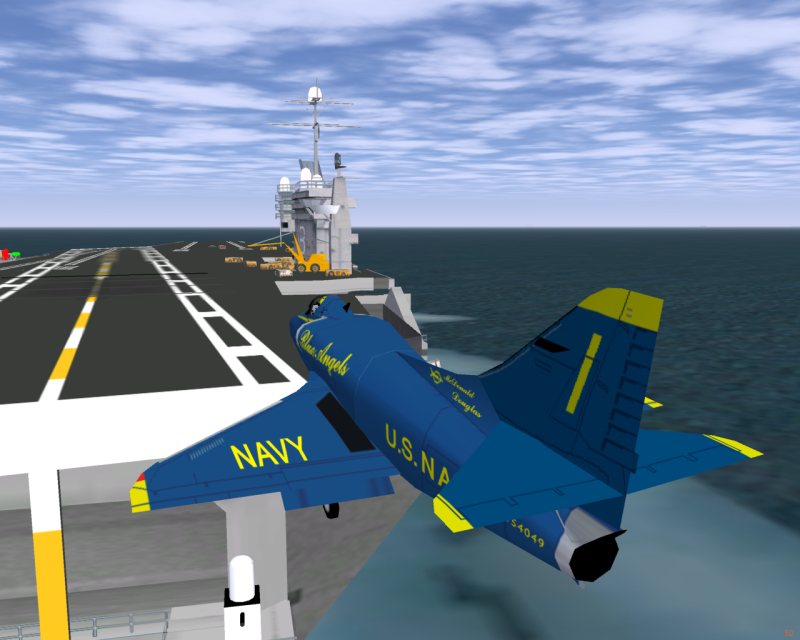
\includegraphics[width=0.5\textwidth]{img/carrier.png}
\caption{A4 landing on the Nimitz\label{carrier}}
\end{figure}


\FlightGear{} supports carrier operations on the Nimitz, (located near San Fransisco) and Eisenhower. 
The carriers are equipped with working catapult, arrester wires, elevators, TACAN and FLOLS and 
are currently available for aircraft using the YASim FDM (in particular the Seahawk, Seafire and A4F.)

To enable the carrier, you must edit your preferences.xml file in \$FG\_ROOT using a text editor (e.g. Notepad
under Windows). Search for the word ``nimitz''. You ought to find something that looks like this;

\begin{verbatim}
<!--<scenario>nimitz_demo</scenario>--> 
\end{verbatim}

You should remove the ``comment'' marks so that it looks like this;


\begin{verbatim}
<scenario>nimitz_demo</scenario> 
\end{verbatim}

Also ensure that the line above that referring to ai being enabled is set to "true"

Save the file and quit the text editor.

\subsection{Starting on the Carrier}

You are now ready to start FlightGear. To position your aircraft on the carrier at startup, 
use the following command line options (noting the upper-case "N");

\begin{verbatim}
--carrier=Nimitz --aircraft=seahawk 
\end{verbatim}

Note that several FG aircraft are carrier capable, but the seahawk is possibly the easiest to fly to begin with.

If you are using the Windows or OSX launcher to run FG, you should find a text entry box in the gui that 
allows you to specify command line options, add the above options there. Linux or Cygwin users can just 
add them to their usual startup command: 

\begin{verbatim}
fgfs --carrier=Nimitz --aircraft=seahawk
\end{verbatim}

Please note the uppercase ``N' in ``Nimitz'.

\subsection{Launching from the Catapult}

Once FlightGear has started, you should ensure that the parking brakes are off and press and hold ``L'' to 
engage the launchbar. You must hold down ``L'' until you have successfully launched. 
You should notice the aircraft being pulled into alignment with the catapult and see 
the strops appear and hold down the aircraft.  This will only happen if your aircraft is 
close enough to the correct spot on the catapult; as a rough guide, for the default 
parking position the seahawk's nose should be rougly level with the deck observation bubble.

To get the carrier into as good a position as possible for launch, select the ``ATC/AI'' menu, then 
check the "Turn into wind" box under the ``AI Carrier'' section. You should now notice the carrier 
begin to pick up speed and turn into the wind, and naturally the deck may tilt somewhat as it turns. 
You should wait for this maneuver to finish and the deck to return to level before moving on to the next stage.

Being engaged to the catapult, you should spool up the engines to full power, ensure the brakes are off 
and that all flight controls are in a suitable position for launch (stick held right back with the seahawk.)  
When ready, press ``C'' to release the catapult. Your aircraft will be hurled forward off the deck, and 
you should be able to raise the undercarriage and climb slowly away, being careful to avoid stalling.

\subsection{Finding the Carrier - TACAN}

Actually finding the carrier in a vast expanse of open water can be very difficult, especially if visibility 
is poor. To assist with this task, Nimitz is equipped with TACAN, which allows a suitably-equipped 
aircraft (Seahawk at present) to obtain a range and bearing to the carrier. First, you must set 
the appropriate TACAN channel, 029Y in this case, in the radios dialogue (ctrl-r or choose 
Equipment/Radio Settings from the FG menubar). You should, if within range, notice the DME instrument 
show your distance from the carrier, and the ADF instrument (next to the DME in the seahawk) should 
indicate a bearing to the carrier. Turn to the indicated heading and you should see the DME dial 
indicate your closing in on the carrier.

\subsection{Landing on the Carrier}

This is the most difficult part of the operation, as in real life. You might well find Andy Ross' tutorial on 
operating the A4 Skyhawk useful here. It is available from here:

\noindent
\web{http://www.seedwiki.com/wiki/flight\_gear/a4\_skyhawk.cfm?wpid=209330}

Basically you should use the TACAN to locate the carrier, and 
line up with the rear of the deck. As this part of the deck is at an angle to the course of the vessel, 
you may need to correct your alignment often. Ensure that the aircraft is in the correct configuration for 
approach (the Help/Aircraft Help menu should contain useful data for your aircraft) and that the gear and 
the arrestor hook are down.

As you approach you should see, on the left hand side of the deck, a set of brightly coloured lights - called 
the Fresnel Lens Optical landing System (FLOLS). This indicates your position on the landing glideslope. 
You will see a horizontal row of green lights, and when approximately on the glideslope, an orange light 
(known in some circles as the ``meatball'') approximately in line with the green lights. When approaching 
correctly, the meatball appears in line with the green lights. If you are high it is above, and when low 
it is below. If you are very low the meatball turns red. If you fly to keep the meatball aligned you 
should catch number 3 wire.

Carrier landings are often described as ``controlled crashes'' and you shouldn't waste your time attempting 
to flare and place the aircraft gently on the deck like you would with a conventional landing - ensuring that 
you catch the wires is the main thing.

Immediately your wheels touch the deck, you should open the throttles to full power, in case you have 
missed the wires and need to ``go around'' again; the wires will hold the aircraft if you have caught them, 
even at full power.

If you wish, you can then (with 0.9.10 and later) raise the elevators from the ATC/AI menu, taxy onto one of the elevators, 
lower it (uncheck the box on the menu) and taxy off into the hangar.

Don't be discouraged if you don't succeed at first - it's not an easy maneouver to master. If after a little 
practice you find the Seahawk too easy, you could move on to the Seafire for more of a challenge! 


\section{Atlas\label{Atlas}}\index{Atlas}

Atlas is a "moving map" application for FlightGear. It displays the aircraft in relation to the terrain below, 
along with airports, navigation aids and radio frequencies. 

Further details can be found on the Atlas website:

\noindent
\web{http://atlas.sourceforge.net}

\section{Multiplayer}\index{Multiplayer}

\FlightGear{} supports a multiplayer environment, allowing you to share the air with other flight-simmers. 
For server details and to see who is online (and where they are flying), have a look at the excellent multiplayer map, available from

\noindent
\web{http://mpmap01.flightgear.org}

Click on the `server' tab to see a list of multiplayer servers. At time of writing there are two sets - one for official \FlightGear{} releases,
and one for the current development stream (CVS). The servers within each set are connected. 
\subsection{Quick Start}

To connect to a server, note down the server name (usually mpserver0?.flightgear,org) and port number (usually 5000) for the appropriate 
server
closest to you, and start \FlightGear{} as follows.

\subsubsection{Using the FlightGear Launcher}

The final screen of the FlightGear Launcher has a section for Multiplayer. 
Simply select the checkbox, enter the hostname and port 
number you noted above and choose a callsign to identify yourself. 
Your callsign can be up to 7 characters in length. 
You must also check The AI models checkbox under Features to make other aircraft visible.

\subsubsection{Using the Command Line}

The basic arguments to pass to fgfs for multiplayer are these:

\begin{verbatim}
--multiplay=out,10,<server>,<portnumber>
--multiplay=in,10,<client>,<portnumber>
--callsign=<anything>
--enable-ai-models
\end{verbatim}

Where 
\begin{enumerate}
\item <portnumber> is the port number of the server e.g. 5000.
\item <server> is the name of the multiplayer server e.g. mpserver01.flightgear.org.
\item <client> is the name of your computer, or the IP address ip address of the network interface being used by FG to connect to the server -
even if that's a local 192.168 type address. e.g. 192.168.0.1
\item <callsign> is the call sign to identify yourself, up to 7 characters, e.g. N-FGFS.
\end{enumerate}

Once the simulator has loaded, you should see yourself displayed on the map. If you don't, check the console for error messages and see the
Troubleshooting section below.

\subsection{Troubleshooting}

To get multiplayer to work, we need information about the IP address of our computer and the ability to communicate with the server. 
How to get this information depends on your configuration and is described below.


\subsubsection{Those using a USB modem to connect to the Internet}

First of all, you need to know the IP address of the network interface you're going to be running FG multiplayer over. 
If your Internet connection is via an ADSL modem that plugs directly into your computer with a USB connection, you 
should be able to find your IP address by visiting http://www.whatismyip.com . Please note that this address may very well 
change every now and again - if MP stops working, check this first.

\subsubsection{Those using some kind of Ethernet router to connect to the Internet}

Otherwise, your connection is likely via some kind of router that connects to your computer via an RJ-45, or "Ethernet" connector 
(similar shape to most Western telephone plugs), or by a wireless link. You need to find the IP address of that network interface.

Under linux, this can be found by logging in as root and typing "ifconfig". You may find more than one interface listed, 
beginning with "lo" - ignore that one. You should have something like "eth0" or "wlan0" also listed - look through this block 
of text for "inet addr". This will be followed directly by the number you're looking for, e.g. "inet addr:192.168.0.150"

Under Windows XP, click start, run, and type "cmd". In the terminal window which appears, type "ipconfig" 
This should show you your IP address - note it down.

With Windows 98, click start, run, and type "winipcfg" to get information about your IP address.

\subsubsection{Configuring your router}

This section ought to be unnecessary now with recent versions of the FG server.  If you have problems though, 
it won't hurt to follow through.

Now, all(!) that remains is to configure your router to forward UDP port 5000 or 5002 to the IP address you've just found. 
This is not something that can be described in step-by-step detail, because each manufacturer's configuration interfaces 
differ greatly. Some tips are given here - if you get stuck, ask nicely on the FlightGear IRC channel for help (details 
on the flightgear website).

You should know how to log on to your router's configuration page, usually via a web browser. You are looking for settings 
pertaining to "port forwarding" "virtual server" "Forwarding Rules" or similar. When you have found the relevant settings, 
you need to add a rule that forwards port 5000 or 5002 (depending on which server you wish to join - add both if you like) 
to the IP address you discovered earlier. If there is a choice given, ensure it is UDP ports that are forwarded. If there 
is no choice, you may assume that both TCP and UDP are being forwarded. Save your configuration, and most routers will 
probably then need to be rebooted to apply the changes.

Note: (for BSD users) If you are using a ADSL modem, you might have to put the port forward command into the ppp.conf 
file rather than firewall. This is because the firewall script will only run each time the machine is booted rather 
than the ppp line coming back online.

\subsubsection{Starting Multiplayer FlightGear}

Finally, start FG using the command line given right at the start (if you're using the windows launcher you will 
find entry boxes for Multiplayer arguments - insert the relevant details there). You will end up with something like this;

\begin{verbatim}
fgfs --callsign=MyName 
     --multiplay=in,10,192.168.0.2,5000   
     --multiplay=out,10,202.83.200.172,5000 
     --enable-ai-models
\end{verbatim}

The current server IP address (in the "out" section) can be found by asking on the IRC channel, and likewise the 
relevant port number; 5000 is the default. Choose your own callsign - this is currently limited to seven characters.

Once you have started FG, you should, if others are flying, see messages in the terminal from which FG was started, similar to the following;

\begin{verbatim}
Initialising john51a using 'Aircraft/ufo/Models/ufo.xml'  
FGMultiplayRxMgr::ProcessRxData - Add new player. IP: 10.0.0.36,  
Call: john51a,model: Aircraft/ufo/Models/ufo.xml 
\end{verbatim}

The MultiPlayer Map is available at \web{http://mpmap01.flightgear.org} - 
this should show you if anyone else is currently flying, and where.

\subsubsection{If It Still Doesn't Work}

You MUST give your local, behind-the-router IP address for MultiPlayer to work. Trust me on this one!

You should check that your firewall is not causing problems - either turn it off temporarily or add an exception 
to allow incoming connections on port 5000 and 5002.

If it's still just not working for you, ask nicely on the FlightGear IRC channel and someone should be able to assist. 

\section{Multiple Displays}\index{Multiple Displays}

\FlightGear{} allows you to connect multiple instances of the program together
to display different views of the simulation though a highly flexible I/O
subsystem.

For example, you may want to have the aircraft panel displayed on a screen
right infront of you, while the view forward is displayed on a separate screen
or using a projector. Using multiple displays can vastly improve the realism
of the simulation.

Given enough hardware, you can create sophisticated simulation environments
with mock-up cockpits, panels, multiple views, and even a separate control
station allowing an
instructor to fail instruments, change the weather etc. An example of this is
the 747 cockpit project.


\noindent
\web{http://www.flightgear.org/Projects/747-JW/}

\subsection{Hardware}

Each instance of \FlightGear{} can support a single display. Due to the
complexity of the FDM and graphics, \FlightGear{} is very processor-intensive,
so running multiple instances of \FlightGear{} on a single machine is not
recommended.

You will therefore need a computer for each view of the simulation you wish
to display, including the panel. The computers obviously must be networked
and for simplicity should be on the same subnet.

One computer is designated as the master. This computer will run the FDM and
be connected to controls such as yokes, joysticks and pedals. As the machine is
running the FDM, it usually only displays a simple view, typically the main
panel, to maximize performance.

All other computers are designated as slaves. They are purely used for display
purposes and receive FDM information from the master.

\subsection{Basic Configuration}

Creating a basic configuration for multiple displays is straightforward. The
master computer needs to broadcast the FDM and control information to the slaves.
This is done using the following command line options:

\begin{verbatim}
--native-fdm=socket,out,60,,5505,udp
--native-ctrls=socket,out,60,,5506,udp
\end{verbatim}

The slave computers need to listen for the information, and also need to have
their own FDMs switched off:

\begin{verbatim}
--native-fdm=socket,in,60,,5505,udp
--native-ctrls=socket,in,60,,5506,udp
--fdm=null
\end{verbatim}

\subsection{Advanced Configuration}

The options listed above will simply show the same view on both machines. You will probably also want to set the
following command-line options on both master and slave computers.

\begin{verbatim}
--enable-game-mode  (full screen for glut systems)
--enable-full-screen (full screen for sdl or windows)
--prop:/sim/menubar/visibility=false (hide menu bar)
--prop:/sim/ai/enabled=false (disable AI ATC)
--prop:/sim/ai-traffic/enabled=false (disable AI planes)
--prop:/sim/rendering/bump-mapping=false
\end{verbatim}

If using the master computer to display a panel only, you may wish to create a full-screen panel for the
aircraft you wish to fly (one is already available for the Cessna 172), and use the following options.

\begin{verbatim}
--prop:/sim/rendering/draw-otw=false (only render the panel)
--enable-panel
\end{verbatim}

For slave computers displaying side-views, use the following options.

\begin{verbatim}
--fov=35
--prop:/sim/view/config/heading-offset-deg=-35
--prop:/sim/view/config/pitch-offset-deg=3
\end{verbatim}

\section{Recording and Playback}\index{Playback}

Another feature of the I/O system is the ability to record your flight for
later analysis or playback. Technical details of how to record specific FDM
information can be found in the \$FG\_ROOT/protocol/README.protocol file.

To record a flight, use the following command line options:

\begin{verbatim}
--generic=file,out,20,flight.out,playback
\end{verbatim}

This will record the FDM state at 20Hz (20 times per second), using the playback
protocol and write it to a file flight.out.

To play it back later, use the following command line options:

\begin{verbatim}
--generic=file,in,20,flight.out,playback
--fdm=external
\end{verbatim}

The playback.xml protocol file does not include information such as plane type,
time of day, so you should use the same set of command line options as you
did when recording.

\section{Text to Speech with Festival}\index{Text To Speech}

\FlightGear{} supports Text To Speech (TTS) for ATC and tutorial messages through the festival TTS
engine (\web{http://www.cstr.ed.ac.uk/projects/festival/}). This is available on many Linux distros,
and can also be installed easily on a Cygwin
Windows system. At time of writing, support on other platforms is unknown.

\subsection{Installing the Festival system}

\begin{enumerate}
\item Install festival from \web{http://www.cstr.ed.ac.uk/projects/festival/}

\item Check if Festival works. Festival provides a direct console interface. Only the relevant lines are 
shown here. Note the parentheses!

\begin{verbatim}
$ festival
festival> (SayText "FlightGear")
festival> (quit)
\end{verbatim}

\item Check if MBROLA is installed, or download it from here: 

\web{http://tcts.fpms.ac.be/synthesis/mbrola/} 

See under "Downloads"m "MBROLA binary and voices" 
(link at the bottom; hard to find). Choose the binary for your platform. Unfortunately, there's no 
source code available. If you don't like that, then you can skip the whole MBROLA setup. 
But then you can't use the more realistic voices. See below for details of more voices.
Run MBROLA and marvel at the help screen. That's just to check if it's in the path and executable.

\begin{verbatim}
$ mbrola -h
\end{verbatim}
\end{enumerate}

\subsection{Running FlightGear with Voice Support}

First start the festival server:

\begin{verbatim}
$ festival --server
\end{verbatim}

Now, start \FlightGear{} with voice support enabled. This is set through the
/sim/sound/voices/enabled property. You can do this through the command line as follows.

\begin{verbatim}
$ fgfs --aircraft=j3cub \
       --airport=KSQL \
       --prop:/sim/sound/voices/enabled=true
\end{verbatim}

Of course, you can put this option into your personal configuration file. 
This doesn't mean that you then always have to use FlightGear together with Festival. 
You'll just get a few error messages in the terminal window, but that's it. You cannot enable
the voice subsystem when FlightGear is running.

To test it is all working, contact the KSFO ATC using the ' key. You should hear "your" 
voice first (and see the text in yellow color on top of the screen), then you should hear 
ATC answer with a different voice (and see it in light-green color).

ou can edit the voice parameters in the preferences.xml file, and select different screen colors 
and voice assignments in \$FG\_ROOT/Nasal/voice.nas. The messages aren't written to the 
respective /sim/sound/voices/voice[*]/text properties directly, but rather to aliases 
/sim/sound/voices/{atc,approach,ground,pilot,ai-plane}.

\subsection{Troubleshooting}

On some Linux distros, festival access is restricted, and you will get message like the following. 

\begin{verbatim}
client(1) Tue Feb 21 13:29:46 2006 : \
  rejected from localhost.localdomain 
not in access list
\end{verbatim}

Details on this can be found from:

\web{http://www.cstr.ed.ac.uk/projects/festival/manual/festival\_28.html\#SEC130}.

You can disable access restrictions from localhost and localhost.localdomain by adding
the following to a .festivalrc file in \$HOME:
\begin{verbatim}
(set! server_access_list '("localhost"))
(set! server_access_list '("localhost.localdomain"))
\end{verbatim}

Or, you can just disable the access list altogether:

\begin{verbatim}
(set! server_access_list nil)
\end{verbatim}

This will allow connections from anywhere, but should be OK if your machine is behind a
firewall.

\subsection{Installing more voices}

I'm afraid this is a bit tedious. You can skip it if you are happy with the default voice. 
First find the Festival data directory. All Festival data goes to a common file tree, 
like in FlightGear. This can be /usr/local/share/festival/ on Unices. We'll call that 
directory \$FESTIVAL for now.

\begin{enumerate}
\item Check which voices are available. You can test them by prepending "voice\_":

\begin{verbatim}
$ festival
festival> (print (mapcar (lambda (pair) (car pair)) \
                                    voice-locations))
(kal_diphone rab_diphone don_diphone us1_mbrola \
                   us2_mbrola us3_mbrola en1_mbrola)
nil
festival> (voice_us3_mbrola)
festival> (SayText "I've got a nice voice.")
festival> (quit)
\end{verbatim}

\item Festival voices and MBROLA wrappers can be downloaded here: 

\web{http://festvox.org/packed/festival/1.95/}  

The "don\_diphone" voice isn't the best, 
but it's comparatively small and well suited for "ai-planes". If you install it, 
it should end up as directory \$FESTIVAL/voices/english/don\_diphone/. 
You also need to install "festlex\_OALD.tar.gz" for it as \$FESTIVAL/dicts/oald/ and 
run the Makefile in this directory. (You may have to add "--heap 10000000" to the 
festival command arguments in the Makefile.)

\item Quite good voices are "us2\_mbrola", "us3\_mbrola", and "en1\_mbrola". For these you need to 
install MBROLA (see above) as well as these wrappers: festvox\_us2.tar.gz, festvox\_us3.tar.gz, 
and festvox\_en1.tar.gz. They create directories \$FESTIVAL/voices/english/us2\_mbrola/ etc. 
The voice data, however, has to be downloaded separately from another site:

\item MBROLA voices can be downloaded from the MBROLA download page (see above). 
You want the voices labeled "us2" and "us3". Unpack them in the directories that 
the wrappers have created: \$FESTIVAL/voices/english/us2\_mbrola/ and likewise for "us3" and "en1".

\end{enumerate}

\section{Air-Air Refuelling (AAR; feature available past 0.9.10)}
  \index{Air-Air Refuelling}

\subsection{What's possible}

At present, there are two tanker aircraft (KC135-E and KA6-D) and three
receiving aircraft (A4F, Lightning and T38) capable of in-air
refuelling.  When flying one of these aircraft in the default scenery
area, one can locate the tanker aircraft using air-air TACAN and/or
radar and then receive a full or partial load of fuel by flying in
close formation behind the tanker.  Refuelling is also possible between
aircraft in a MultiPlayer session. The KC135 is a boom refueller, while
the KA6 has a hose. The A4F and Lightning are both fitted with a probe
for hose refuelling while the T38 is fitted with a boom receiver. At
the moment, either type can refuel from any tanker, but in the future
it is likely that the correct type will have to be used.

\subsection{Necessary preparations}

Like the aircraft carriers, AAR is implemented as an "AI scenario". 
Selecting these normally requires editing the "preferences.xml" file in
the flightgear data directory.

There is a shortcut in this case though; simply selecting the
Lightning, A4F or T38 should automatically load a scenario containing a
tanker, assuming you haven't changed anything in your preferences.xml
file.

Assuming this is the case, choose one of the aforementioned aircraft,
make sure that "AI models" are enabled and start at KSFO (the default
airport.)

Depending on the scenario, you might see the tanker crossing overhead
when the sim starts; if not, don't worry.

\subsection{In the cockpit}

Perhaps the first thing to do after starting the engines if necessary
is to select the appropriate TACAN channel if your aircraft is so
equipped (the A4F and Lightning both are).  For the KC135 (by default
used by the Lightning and T37) this is currently "040X", and for the
KA6D (used by the A4F) it is "050X".  Enter this channel using the
relevant dropdown boxes in the "radios" dialogue (from the menus,
"equipment/radios" or press control-r).

You should now see the current bearing to the tanker indicated in the
nav display of the A4 or the TACAN indicator (green needle) in the
Lightning.  If the tanker is within range, it will also appear on the
radar display of the T38 or Lightning.  Take off...

\subsection{In the Air}

Turn to an appropriate heading, guided by the TACAN bearing (you should
try a "leading" approach to close in on the tanker) and look for the
tanker on the radar or nav. screen.  Around 5nm away, you should reduce
your speed to around 20kts faster than the tanker (these fly at 280 kts
TAS) - a "slow overtake".  The KC135 will be visible from about 10nm,
the KA6-D, being smaller, just over 1 nm.  You should use airbrakes as
necessary to keep control of your speed should you find yourself
overshooting.

Close to within 50ft of the tanker (don't get too close, or visual
artifacts might hide the boom from view).  You should see indication in
the cockpit that you are receiving fuel - there is a green light in the
A4 fuel gauge, and you should see the indicated tank load increase.

Getting to this stage is not necessarily easy - it can take a lot of
practice.  As with carrier landings, this is not an easy manoeuver in
real life either and there are additional complications in the sim; the
tanker, being an AI model, is unaffected by the wind and flies TAS
(True Air Speed), while you are flying IAS (Indicated Air Speed) and
are affected by the environment.  As in real life, your aircraft will
also steadily increase in weight as the tanks fill which will affect
the trim of the aircraft. (You might find it helpful to use the
autothrottle to help control your speed - ctrl-a then Page Up/Down to
increase and decrease the set speed.)

Once your tanks are full, or you have taken as much fuel as you wish,
close the throttle a little, back away from the tanker and continue
your intended flight.

\subsection{More advanced topics}

\begin{enumerate}

\item Multiplayer Refuelling

Refuelling is possible within a MultiPlayer session given certain
conditions.  A basic flyable KC135 model is available - the pilot of
this aircraft should use the callsign "MOBIL1", "MOBIL2" or "MOBIL3". 
Other numbers are acceptable, but only these three have A-A TACAN
channels assigned.  These are 060X, 061X and 062X respectively.

If the receiving aircraft uses a YASim FDM, there are no further
complications.  Should the receiving aircraft be JSBSim based, the user
must make sure that there are no AI tankers in their configuration. 
This means disabling (commenting out) all refuelling "scenarios" in the
relevant aircraft-set.xml and in preferences.xml.

MP refuelling works in exactly the same way as AI refuelling and is a
fun challenge.  It is best to ensure that your network connection is as
free from interruptions as possible; the MP code does a degree of
prediction if there is a "blip" in the stream of packets and this can
make close formation flight very difficult or even impossible.

\item Selecting Different Scenarios

There are several AAR scenarios available in the AI directory:
\begin{enumerate}
\item refueling\_demo.xml has a KC135 circling near KSFO at 3000ft,
\item refueling\_demo\_1.xml the KC135 on a North/South towline at 8000ft and
\item refueling\_demo\_2.xml the KA6D on a similar N/S path but at 8500ft.
\end{enumerate}

These can be selected by editing preferences.xml (use your operating
system's search facility to locate this if you don't know where it is). 
Open preferences.xml in a text editor (e.g. notepad if on windows) and
search for the <ai> </ai> tags.  Place a line like
\begin{verbatim}
<scenario>refueling\_demo</scenario>
\end{verbatim}
somewhere within the <ai> tags; you should see other scenarios already
there too, perhaps commented out (i.e. with <!-- -->).

\end{enumerate}

%% Revision 0.00  2006/01/01  Stuart
%% Initial revision for version 0.9.9.
